\documentclass{beamer}
\usetheme{Singapore}
\usepackage{changepage}

%\usepackage{pstricks,pst-node,pst-tree}
\usepackage{amssymb,latexsym}
\usepackage{tikz}
\usepackage{graphicx}
\usepackage{fancyvrb}
\usepackage{hyperref}
\usepackage{fancybox}
\usepackage[listings]{tcolorbox}

\definecolor{codegreen}{rgb}{0,0.6,0}
\definecolor{codegray}{rgb}{0.5,0.5,0.5}
\definecolor{codepurple}{rgb}{0.58,0,0.82}
\definecolor{backcolour}{rgb}{0.95,0.95,0.92}

\lstdefinestyle{mystyle}{
    language=Python,
    backgroundcolor=\color{backcolour},   
    commentstyle=\color{codegreen},
    keywordstyle=\color{magenta},
    numberstyle=\tiny\color{codegray},
    stringstyle=\color{codepurple},
    basicstyle=\ttfamily\footnotesize,
    breakatwhitespace=false,         
    breaklines=true,                 
    captionpos=b,                    
    keepspaces=true,                 
    numbers=left,                    
    numbersep=5pt,                  
    showspaces=false,                
    showstringspaces=false,
    showtabs=false,                  
    tabsize=2,
    escapechar=|,
    frame=single
}

\lstset{style=mystyle}


\newcommand{\bi}{\begin{itemize}}
\newcommand{\li}{\item}
\newcommand{\ei}{\end{itemize}}
\newcommand{\Show}[1]{
\begin{center}
\shadowbox{\begin{minipage}{0.8\textwidth}
          #1
          \end{minipage}}
\end{center}
}
\newcommand{\arrow}{\ensuremath{\rightarrow}}

\newcommand{\uparr}{\ensuremath{\uparrow}}


\newcommand{\fig}[2]{\centerline{\includegraphics[width=#1\textwidth]{#2}}}

\newcommand{\bfr}[1]{\begin{frame}[fragile]\frametitle{{ #1 }}}
\newcommand{\efr}{\end{frame}}

\newcommand{\cola}{\begin{columns}\begin{column}{0.5\textwidth}}
\newcommand{\colb}{\end{column}\begin{column}{0.5\textwidth}}
\newcommand{\colc}{\end{column}\end{columns}}


\title{Think Python 2e, Chapter 18 Notes}
\author{Inheritance}

\begin{document}

\begin{frame}
\maketitle
\end{frame}

\bfr{Card objects}

\cola
Encoding of suits:\\

\begin{tabular}{rcl}
Spades & $\rightarrow$ & 3\\
Hearts & $\rightarrow$ & 2\\
Diamonds & $\rightarrow$ & 1\\
Clubs & $\rightarrow$ & 0\\
\end{tabular}
\colb
Encoding of ranks:\\

\begin{tabular}{rcl}
Ace & $\rightarrow$ & 1\\
...\\
Jack & $\rightarrow$ & 11\\
Queen & $\rightarrow$ & 12\\
King & $\rightarrow$ & 13\\
\end{tabular}
\colc

\end{frame}

\bfr{Class definition of card:}
\begin{lstlisting}
class Card:
    """Represents a standard playing card."""

    def __init__(self, suit=0, rank=2):
        self.suit = suit
        self.rank = rank
\end{lstlisting}
\begin{lstlisting}
queen_of_diamonds = Card(1, 12)
\end{lstlisting}

\end{frame}

\bfr{Class attributes}
\begin{lstlisting}
# inside class Card:

suit_names = ['Clubs', 'Diamonds', 'Hearts', 'Spades']
rank_names = [None, 'Ace', '2', '3', '4', 
              '5', '6', '7', '8', '9', '10',
              'Jack', 'Queen', 'King']

def __str__(self):
    return '%s of %s' % (Card.rank_names[self.rank],
                         Card.suit_names[self.suit])

\end{lstlisting}
\bi
\li Variables declared inside a class but outside of any
method, like \lstinline{suit_names} and \lstinline{rank_names}
 are {\bf class variables}.
\li They are associated with the class \lstinline{Card}
\li Variables like \lstinline{suit} and \lstinline{rank} are 
{\bf instance variables}
\ei

\end{frame}
\bfr{Creating cards}
\begin{lstlisting}
>>> card1 = Card(1, 11)
>>> print(card1)
Jack of Diamonds
\end{lstlisting}

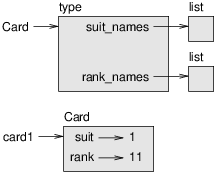
\includegraphics{statediagram18-1}

\end{frame}



\end{document}
